\documentclass[]{IEEEtran}

\title{Modellazione di un Moltiplicatore Floating-point Single Precision in SystemC TLM ed Integrazione in una Virtual Plaform}
\author{Elena Ramon}

\usepackage{graphicx}
\usepackage[italian]{babel}
\usepackage{blindtext}
\usepackage{enumitem}
\usepackage{caption}
\captionsetup{tableposition=top,figureposition=bottom,font=small}

\begin{document}
	\maketitle
	
	\begin{abstract}
		Questo documento presenta l'implementazione di un sistema per il calcolo della moltiplicazione in virgola mobile nei diversi stili di codifica di SystemC TLM e presenta un'implementazione su Virtual Platform.
	\end{abstract}
		
	\section{Introduzione}
	
	I sistemi descritti nel documento rappresentano il calcolo della moltiplicazione in virgola mobile nei diversi stili di codifica di SystemC TLM e su una Virtual Platform.

	\subsection{Virtual Platform}

	L'obiettivo \`e quello di osservare come un sistema interagisce con l'architettura sottostante. 

	Si \`e cercato di integrare il sistema sviluppato nel progetto precedente in una piattaforma virtuale dove sono presenti anche altri componenti. 
	
	I moduli principali che sono stati aggiunti nella directory platform sono:
	\begin{itemize}
		\item il wrapper del modulo moltiplicatore in virgola mobile, il quale si occupa di definire:
		\begin{itemize}
			\item in quale modo vengono recepiti gli input dal bus e quando passarli al modulo;
			\item in quale modo vengono recepiti gli output del modulo e quando passarli al bus.
		\end{itemize}
		\item il moltiplicatore stesso, con alcune modifiche rispetto alla precedente implementazione.
	\end{itemize}	

	\subsection{SystemC TLM}

	L'obiettivo \`e quello di osservare le caratteristiche delle diverse implementazioni anche a confronto tra loro.

	SystemC TLM viene solitamente utilizzato per una progettazione veloce con poca attenzione ai dettagli di implementazione, quindi pi\`u astratta. Ogni stile di codifica \`e composto da un testbench, che funge da iniziatore della transazione e da un moltiplicatore, che rappresenta il target. Per svilupparli \`e stato preso come riferimento l'esempio presentato in laboratorio, adattandolo al caso specifico in esame.

	I risultati finali, che verranno in seguito analizzati, mostrano come, nonostante la medesima rappresentazione astratta, gli stili di codifica abbiano dei tempi di simulazione differenti, dovuti alle diverse tipologie di relazione tra dati e tempo (la sincronizzazione tra target ed iniziatore). Per eseguire un confronto con il sistema sviluppato a livello RTL nel progetto precedente, quest'ultimo \`e stato modificato in modo tale che venisse eseguita una sola moltiplicazione.
		
	\section{Background}
	
	\subsection{Virutal Platform}
	
	Le Virtual Platform sono una rappresentazione astratta dell'architettura su cui un sistema embedded dovr\`a essere eseguito. Utilizzare una Virtual Platform, per la progettazione del moltiplicatore in virgola mobile, ha permesso di avere pieno controllo dell'hardware su cui il sistema embedded veniva eseguito, consentendo la risoluzione pi\`u rapida di errori attraverso la riproduzione consecutiva dei medesimi passi in fase di test. Un'altra caratteristica fondamentale, che ha permesso di anticipare la fase di sviluppo del sistema in esame, \`e la facilit\`a di estensione e modifica di Virtual Platform pre-esistenti, in questo caso \`e stata utilizzata la piattaforma COM6502-Splatters~\cite{COM6502-Splatters}.
	
	\subsection{SystemC TLM}
	
	SystemC TLM (Transaction Level Modeling)~\cite{SystemC-TLM} permette di modellare le funzionalit\`a di un sistema ad un livello pi\`u astratto, quindi con meno dettagli di implementazione, rispetto all'RTL (Register Transfer Level) ~\cite{RTL}, dando pi\`u importanza alla transazione dei dati (l'interazione tra i moduli).
	Il sistema \`e stato implementato nei tre diversi stili di codifica previsti dallo standard:
	\begin{description}
		\item[Untimed] dove il concetto di temporizzazione di una transazione non \`e considerato;
		\item[Loosely-timed] in cui ogni transazione viene temporizzata solo all'inizio e alla fine della transazione;
		\item[Approximately-timed] in cui ogni transazione viene sincronizzata in pi\`u punti. Nella versione base sono quattro: inzio della richiesta, fine della richiesta, inizio della risposta e fine della risposta.
	\end{description}

	I soggetti che interagiscono in una transazione sono due, l'iniziatore (colui che inizia la transazione) e il target (il punto finale della transazione, colui con cui l'iniziatore vuole interagire). Questi durante la comunicazione si scambiano un payload contenente i dati su cui effettuare operazioni e informazioni di controllo. Lo standard prevede la possibilit\`a di estendere il payload generico per adattarlo ai diversi protocolli che possono essere utilizzati, come avviene nel sistema in esame.
	
	\section{Metodologia applicata}

	\subsection{Virtual Platform}
	
	Come detto nella sezione precedente il moltiplicatore in virgola mobile \`e stato integrato su una Virtual Platform gi\`a esistente, per cui sono state aggiunte funzioni e collegamenti.

	\subsubsection{Application}
	
	Sono stati modificati i seguenti file:
	\begin{itemize}
		\item main.c: \`e stato introdotta la moltiplicazione in virgola mobile, in particolare vengono dichiarate quattro variabili di tipo uint32\_t:
		\begin{itemize}
			\item \textit{VHDL\_in\_1} e \textit{VHDL\_in\_2}: gli operandi per il moltiplicatore in VHDL;
			\item \textit{verilog\_in\_1} e \textit{verilog\_in\_2}: gli operandi per il moltiplicatore in verilog;
		\end{itemize}
		il valore di tre di esse (\textit{VHDL\_in\_1}, \textit{verilog\_in\_1} e \textit{VHDL\_in\_2}) viene definito nel main.c, mentre il valore della quarta (\textit{verilog\_in\_2}) deriva dall'iomodule. Vi sono poi le due variabili, sempre di tipo uint32\_t, per la memorizzazione del risultato.

		Il main esegue una sola chiamata a \textit{floating point multiplication} la funzione definita in routines.c, a cui passa i quattro input e i puntatori ai due output. Una volta ottenuti i risultati chiama la funzione \textit{io\_write()}.
		\item routines.c (con il corrispondente routines.h): viene definita la funzione ``floating\_point\_multiplication''. La dimensione massima dei dati trasportabili sul bus \`e di 32 bit e la lunghezza degli operandi della moltiplicazione in virgola mobile \`e di 32 bit. Per tale motivo si \`e reso necessario fare pi\`u invii consecutivi alla piattaforma. Gli input vengono inviati in modo tale da corrispondere al medesimo ordine del progetto implementato nella precedente consegna (quindi \textit{VHDL\_in\_1}, \textit{verilog\_in\_1}, \textit{VHDL\_in\_2}, \textit{verilog\_in\_2}). Dopo aver inviato gli input la funzione attende che i risultati siano pronti, quindi  li assegna ai puntatori \textit{VHDL\_result} e \textit{verilog\_result}.
	\end{itemize}

	\subsubsection{Platform}
	Sono stati modificati i seguenti file:
	\begin{itemize}
		\item top\_level.v: \`e stata aggiunta la mappatura al modulo per la moltiplicazione in virgola mobile;
		\item tb.v: \`e stato cambiato il valore che viene passato alla richiesta iomodule.
	\end{itemize}

	Sono stati aggiunti i seguenti file:
	\begin{itemize}
		\item floating\_point\_multiplier\_apb\_wrapper.vhd: rappresenta l'interfaccia che permette al modulo che esegue la moltiplicazione in virgola mobile di interagire con il bus a cui \`e collegato sulla porta numero 3. L'applicazione e la piattaforma non sono sincronizzate tra loro, per cui per fare in modo che il modulo riceva gli operatori nel modo corretto \`e stata implementata una EFSM (Extended Finite State Machine), rappresentata in figura~\ref{fig:efsm}. L'applicazione e la piattaforma si sincronizzano sul valore di \textit{penable}, come mostrato nel diagramma di sequenza~\ref{fig:sequence}, e vengono utilizzate tre variabili temporanee, tutte di tipo unsigned su 32 bit, per contenere gli input in fase di acquisizione, in modo tale da passarli al modulo nel modo e al momento corretto, e per contenere gli output, in modo tale da acquisirli dal modulo e inviarli all'applicazione in modo corretto. Il wrapper si occupa anche di eseguire il cast dei valori in ingresso e in uscita dal modulo.

		I segnali che vengono definiti nel wrapper sono:
		\begin{itemize}
			\item \textit{current\_state} e \textit{next\_state}: per rappresentare gli stati della EFSM;
			\item \textit{result}: unsigned su 32 bit;
			\item VHDL\_in e verilog\_in: unsigned su 32 bit per passare i dati al modulo;
			\item \textit{temp}, \textit{temp1}, \textit{temp2}: unsigned 32 bit;
			\item \textit{done} e \textit{ready}: bit usati per sincronizzare il wrapper e il top level del modulo.
		\end{itemize}

		Il mapping tra le porte del wrapper e del moltiplicatore \`e il seguente:
		\begin{itemize}
			\item \textit{clk} nel moltiplicatore corrisponde al \textit{pclk} del wrapper (rispetto alla versione implementata nel precedente progetto, \`e stato cambiato il tipo di dato del clock, da bit a std\_logic);
			\item \textit{ready} nel moltiplicatore corrisponde al \textit{ready} del wrapper;
			\item \textit{VHDL\_in} nel moltiplicatore corrisponde al \textit{VHDL\_in} del wrapper;
			\item \textit{verilog\_in} nel moltiplicatore corrisponde al \textit{verilog\_in} del wrapper;
			\item \textit{eccezione\_out} nel moltiplicatore corrisponde ad \textit{eccezione\_out} del wrapper;
			\item \textit{done} nel moltiplicatore corrisponde al \textit{done} del wrapper;
			\item \textit{result} nel moltiplicatore corrisponde al \textit{result} del wrapper;
			\item \textit{rst} nel moltiplicatore corrisponde al \textit{presetn} del wrapper (come per il clock \`e stato cambiato il tipo di dato rispetto al precedente progetto).
		\end{itemize}
		
		\item I file relativi al modulo per le moltiplicazioni in virgola mobile del precedente progetto:
		\begin{itemize}
			\item top level, definito come floating\_point\_multiplier.vhd;
			\item multiplier vhdl;
			\item multiplier verilog.
		\end{itemize}
	\end{itemize}

	\subsection{SystemC TLM}
	
	Come detto nella sezione precedente il moltiplicatore in virgola mobile \`e stato implementato nelle tre diverse versioni di TLM: approximately-timed, loosely-timed e untimed. Tutte presentano la stessa struttura:
	\begin{itemize}
		\item un testbench che funge da iniziatore
		\item un moltiplicatore che rappresenta il target
	\end{itemize}
	Nel sistema in esame il payload che viene inviato nelle transazioni \`e stato esteso con un puntatore alla struttura iostruct, la quale contiene le informazioni sui dati in input (i due operandi) e output (il risultato). 

	\subsubsection{Untimed}
	Le transazioni avvengono senza il passaggio di riferimenti temporali, la sincronizzazione viene garantita dalla chiamata della primitiva \textit{b\_transport} con interfaccia bloccante. Il testbench richiama la funzione, agganciando il payload, il target riceve la chiamata, esegue la moltiplicazione tra gli operandi e ritorna il risultato.

	\subsubsection{Loosely-timed}
	La comunicazione tra le componenti avviene attraverso la primitiva \textit{b\_transport}, come per ``Untime'', la particolarit\`a di questo stile di codifica \`e il Temporal Decoupling, cio\`e la capacit\`a del testbench di proseguire la sua esecuzione ``al di fuori'' del tempo di simulazione, quindi senza produrre effetti su di esso, finch\'e non raggiunge un punto di sincronizzazione o non termina il tempo a sua disposizione (ogni processo in SystemC TLM viene eseguito per un quanto di tempo).

	\subsubsection{Approximately-timed 4 fasi}
	\`E stata sviluppata la versione base la quale prevede 4 fasi: inizio e fine della richiesta, inizio e fine della risposta. Il testbench chiama la primitiva \textit{nb\_transport\_fw} (inizio della richiesta) per la quale attende una risposta di ricezione da parte del moltiplicatore (fine della richiesta). Quindi il target calcola la moltiplicazione, chiama la primitiva \textit{nb\_transport\_bw} (inizio della risposta) in seguito alla quale l'iniziatore continua la sua esecuzione (fine della risposta).

	Le tre versioni implementano la stessa funzionalit\`a, la moltiplicazioni di due fattori in virgola mobile, la differenza si trova quindi nel tempo di simulazione impiegato da ciascuna. I tempi di simulazione sono presentati nella tabella \ref{tab:time}. 
	
	Per ottenere dei dati rilevanti in ogni tipologia sono state eseguite 10000000 moltiplicazioni. Il modulo RTL presente nella tabella \`e una versione composta da un solo moltiplicatore, in modo da poter essere confrontabile con le versioni in SystemC TLM (quindi rispetto al modulo SystemC RTL presentato nel precedente progetto non \`e presente il top level, in quanto non pi\`u necessario, e viene creata una sola istanza del moltiplicatore la quale comunica direttamente con il testbench).
	
	I dati della tabella rendono evidente che maggiore \`e il controllo del tempo e la sincronizzazione dei processi pi\`u il tempo di simulazione \`e lungo. Nello specifico il dato real time rappresenta il tempo di esecuzione effettivamente impiegato dal calcolatore per terminare l'esecuzione del sistema, il suo valore \`e quindi influenzato da fattori esterni al sistema stesso (include anche il tempo utilizzato da altri processi). Il dato user time rappresenta il tempo impiegato dalla CPU per l'esecuzione effettiva del sistema. Il dato sys time rappresenta il tempo impiegato per l'esecuzione da parte della CPU di system call per il processo. 
	
	\begin{table}[]
		\centering
		\begin{tabular}{lllll}
			& AT4     & LT     & UT    & RTL    \\ \hline
			Real time   & 38m21,518s & 17m27,345s & 15m4,200s & 21m20,212s \\
			User time   & 0m33,111s & 0m19,793s & 0m14,260s & 1m37,117s \\
			System time & 9m43,919s & 5m9,430s & 3m49,961s & 19m41,661s \\ 
			&&&&\\
		\end{tabular}
		\caption{Tempi di esecuzione su 10000000 moltiplicazioni}
		\label{tab:time}
	\end{table}
	
	\section{Risultati}

	Il testbench utilizzato in entrambi i progetti \`e di tipo automatico con verifica lasciata al programmatore. In particolare in Virtual Platform le due moltiplicazioni vengono fatte sugli stessi operandi, mentre in SystemC TLM gli operandi sono tutti diversi.

	\subsection{Virtual Platform}
	Il sistema \`e stato prima implementato aggiungendo alla piattaforma pre-esistente un solo moltiplicatore con il suo wrapper, questo ha permesso di verificare quali accorgimenti fosse necessario prendere al fine di far funzionare il tutto. Infatti il flusso di esecuzione da seguire in un sistema con un solo moltiplicatore \`e pi\`u piccolo, di conseguenza \`e stato possibile sistemare eventuali errori pi\`u velocemente. Dopo aver ottimizzato il sistema con un solo moltiplicatore \`e stato aggiunto tutto il modulo e verificato il corretto funzionamento. Le figure ~\ref{fig:memory-waveform}, ~\ref{fig:io-total}, ~\ref{fig:mul-total} mostrano le waveform della memoria, dell'iomodule e del moltiplicatore, le figure ~\ref{fig:io-waveform} e ~\ref{fig:mul-waveform} sono un ingrandimento delle waveform originali.

	\subsection{SystemC TLM}
	Il sistema \`e stato implementato nelle tre diverse versioni e verificato singolarmente per ciascuna, prima attraverso l'esecuzione di una sola moltiplicazione uguale per tutti gli stili di codifica, quindi con la generazione random dei valori. La verifica della corretta sincronizzazione \`e stata effettuata attraverso l'ordine dei messaggi mostrati durante la simulazione. 

	Il confronto tra i tempi di simulazione dei diversi stili di codifica di SystemC TLM e SystemC RTL conferma il divario tra astrattezza, quindi tempi di simulazione pi\`u brevi (SystemC TLM), e precisione temporale con maggiori dettagli di implementazione, quindi una simulazione pi\`u lenta (SystemC RTL). Nel sistema in esame ritengo che un'implementazione ad un livello di astrazione pi\`u basso possa essere migliore, anche se pi\`u lenta, dato che nella versione RTL sono state prese decisioni riguardo la tipologia di arrotondamento e sono state gestite le eccezioni, mentre nella versione ad alto livello viene eseguita la moltiplicazione semplice, senza valutare tutti questi aspetti che nel caso della virgola mobile sono certamente importanti. Naturalmente se il sistema fosse rivolto ad un mercato con un elevato numero di concorrenti scegliere l'implementazione in SystemC TLM avvantaggerebbe sul TTM (Time To Market), dato che \`e risultato pi\`u veloce e semplice sviluppare tutte e tre le versioni in SystemC TLM piuttosto che quella in SystemC RTL. Un altro fattore che potrebbe influenzare la scelta tra i due livelli di astrazione \`e la reattivit\`a richiesta al sistema, se il tempo \`e un elemento fondamentale per il sistema richiesto la versione pi\`u adeguata \`e quella di SystemC TLM, altrimenti SystemC RTL. 
	
	\section{Conclusioni}
	Lo sviluppo del moltiplicatore in virgola mobile, nei diversi stili di codifica di SystemC TLM, ha permesso di comprendere quali fattori influenzino la scelta tra i diversi livelli di astrazione. 
	
	L'integrazione del modulo implementato nel progetto precedente in una Virtual Platform ha permesso di verificare quale sia l'interazione del sistema con l'architettura sottostante e di esplorare l'architettura durante l'esecuzione.
	
	
	\bibliographystyle{IEEEtran}
	\bibliography{biblio}
	
	\begin{figure*}[bt]
		\centering
		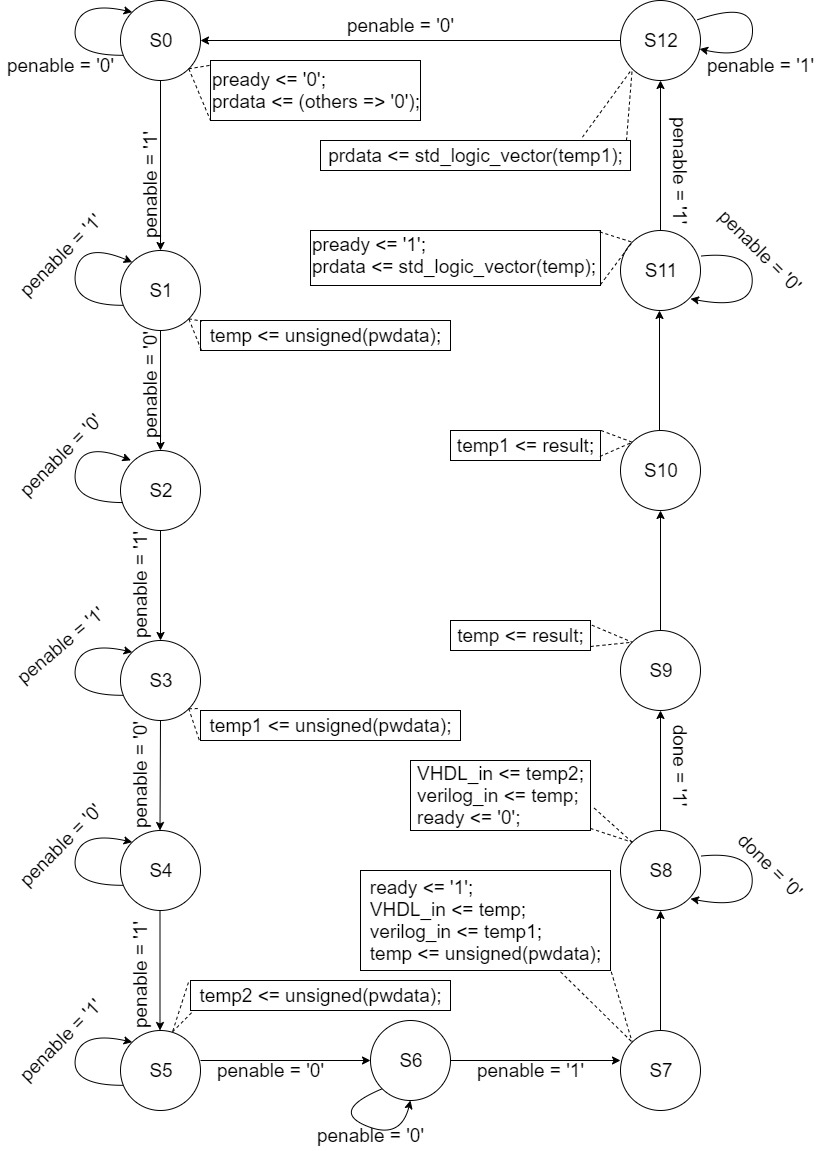
\includegraphics[width=\textwidth]{figures/EFSM}
		\caption{EFSM Floating Point Multiplier Wrapper}
		\label{fig:efsm}
	\end{figure*}

	\begin{figure*}[bt]
		\centering
		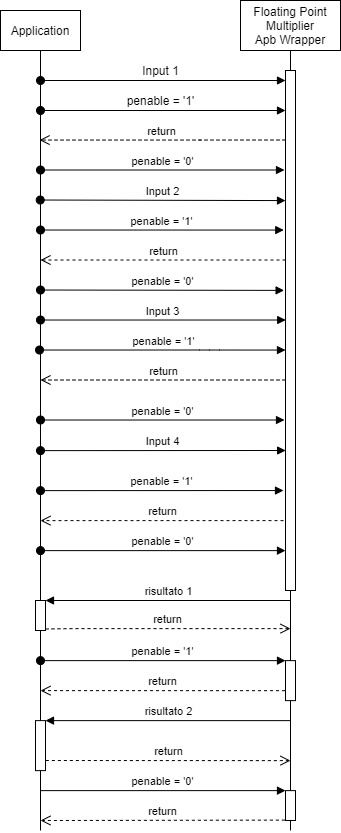
\includegraphics[width=\columnwidth]{figures/sequence}
		\caption{Diagramma di sequenza del protocollo di comunicazione}
		\label{fig:sequence}
	\end{figure*}
	
	\begin{figure}[bt]
		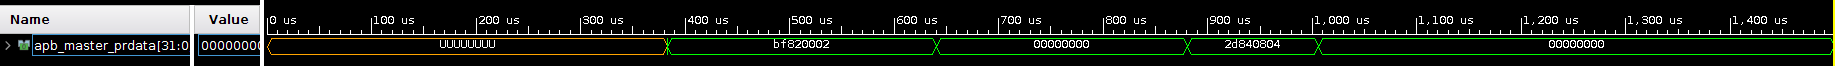
\includegraphics[width=\textwidth]{figures/memory-waveform}
		\caption{Waveform output della memoria}
		\label{fig:memory-waveform}
	\end{figure}

	\begin{figure}[bt]
		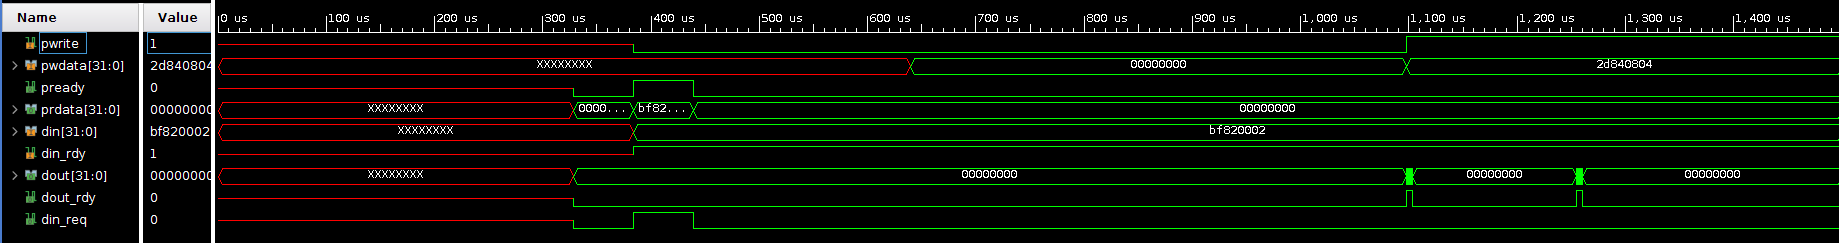
\includegraphics[width=\textwidth]{figures/io-total}
		\caption{Waveform modulo moltiplicatore}
		\label{fig:io-total}
	\end{figure}

	\begin{figure}[bt]
		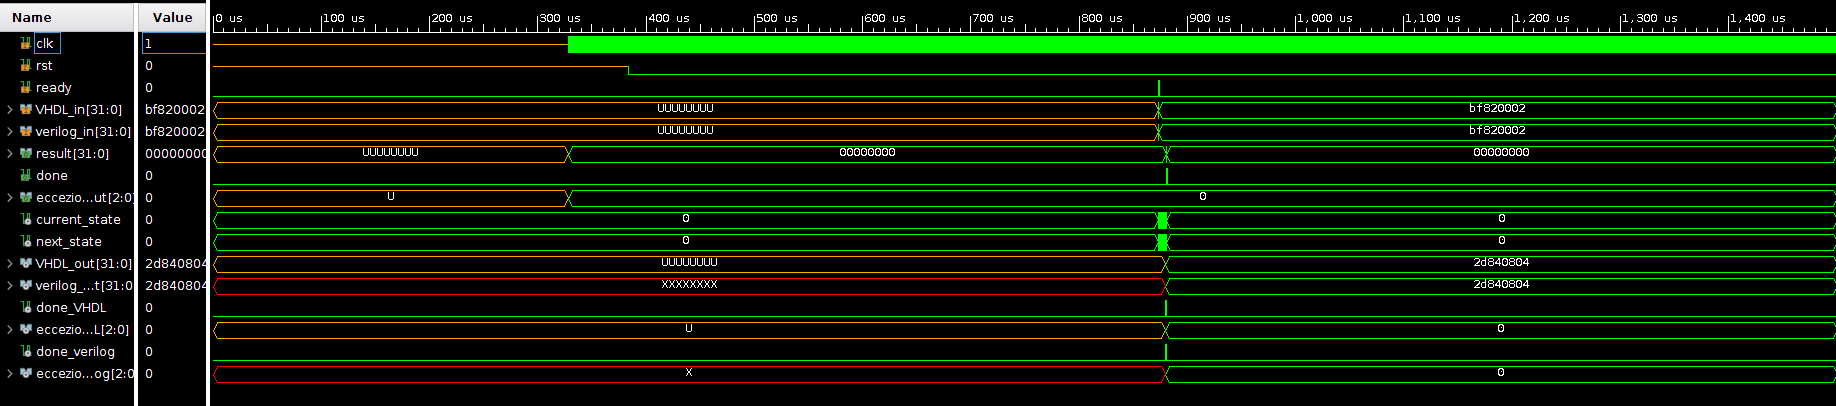
\includegraphics[width=\textwidth]{figures/mul-total}
		\caption{Waveform modulo moltiplicatore}
		\label{fig:mul-total}
	\end{figure}
	
	\begin{figure}[bt]
		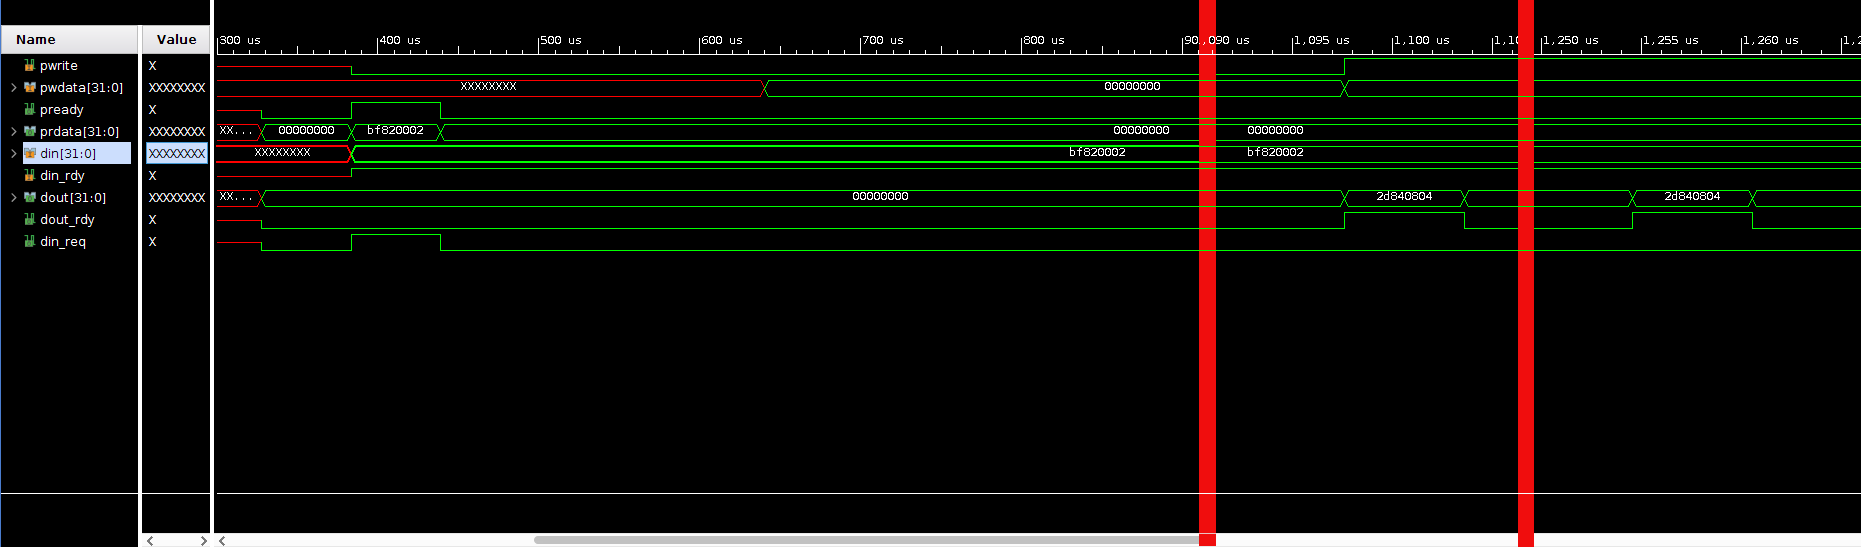
\includegraphics[width=\textwidth]{figures/io-waveform}
		\caption{Ingrandimento waveform modulo I/O}
		\label{fig:io-waveform}
	\end{figure}
	
	\begin{figure}[bt]
		\includegraphics[width=\textwidth]{figures/mul-waveform}
		\caption{Ingrandimento waveform modulo moltiplicatore}
		\label{fig:mul-waveform}
	\end{figure}
	
\end{document}